\documentclass[11pt]{article}
\usepackage{graphicx}
\usepackage{hyperref}
\usepackage{natbib}
\usepackage{indentfirst}
\setlength{\textwidth}{6.5in}
\setlength{\headheight}{0in}
\setlength{\textheight}{8.0in}
\setlength{\hoffset}{0in}
\setlength{\voffset}{0in}
\setlength{\oddsidemargin}{0in}
\setlength{\evensidemargin}{0in}
\usepackage{amsmath}
\title{Krishna's First Problem Set}
  
\author{Krishna N. Dindial}


\begin{document}

\maketitle


\section{Problem 1}
We start with the number 100.98763 and are asked to evaluate the number its 32 bit float representation actually corresponds to.
First I used Michael Blanton's "getbits" code from class. Once I had the bits, I wanted to represent the number as a fraction. The formula for the mantissa is: 

\begin{equation}
\text{Mantissa} = 1 + \sum_{i=1}^{23} b_i \cdot 2^{-i}
\end{equation}

I want to get everything in a common denominator, so instead I can write the sum as: 


\begin{equation}
\text{Mantissa} = \frac{2^{23}}{2^{23}} + \sum_{i=1}^{23} b_i \cdot \frac{2^{22-i}}{2^{23}}
\end{equation}

Using the above formula, I calculated that the numerator of the mantissa was: 13236651, so to get the full mantissa you just divide that by $2^{23}$. I then calculated that the exponent term is $2^6$ so the final number should be:

\begin{equation}
    \frac{2^6*13236651}{2^{23}}
\end{equation}

which is 
\begin{equation}
    \frac{13236651}{2^{17}}
\end{equation}

I evaluated this fraction as a np.float64, and it gives me: 100.98763275146484. Our original number is 100.98763, so our calculated number at 64 bit precision differs by 0.00000275146484.



\section{Problem 2}

from equation 1, we can see that the smallest number we can add to 1 is $2^{-23}$ in 32 bit precision. For a float 64, there are 52 bits for the mantissa, so the  smallest number you can add to 1 is $2^{-52}$.
\par
In either of these representations, the largest number you could represent without an overflow has a 0 in the sign bit, zero in the last bit of the exponent, and 1s every were else. In 32 bit floating point representation where we have 8 bits in the exponent and 23 bits in the mantissa,  This corresponds to $2^{2^7}*(2-2^{-23})$ which is approximately: 3.4028235e+38. In 64 bit representation where we have 11 bits for the exponent and 52 bits in the mantissa, the largest number you could represent would be $2^{127}*{2-2^{1023}}$ which is approximately 1.7976931348623157e+308. 
\par
the smallest positive number you could represent would have all zeros everywhere except the last bit of the mantissa. In 32 bit, this would correspond to $2^{-127}*(1+2^{23}$ which is approximately 1.175494490952134e-38. In 64 bit precision, this corresponds to $2^{-1023}*(1+2^{52}$ which is approximately 1.1125369292536007e-308.

\section{Problem 3}
For an L of 100, I calculated that M is approximately -1.7418198. Timit calculated it takes about 14.5 s with a for loop and without a for loop, it code takes about .5 seconds. Both seem very high for just one run.

\section{Problem 4}

Here is my mandelbrot plot!:

\begin{figure}[h!]
    \centering
    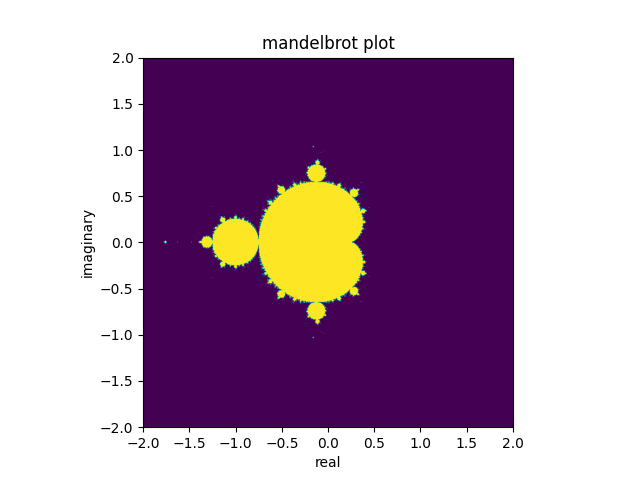
\includegraphics[width=0.5\linewidth]{mandelbrotPlot.png}
    \caption{Cool!}
    \label{fig:enter-label}
\end{figure}

I used chatgpt twice. The first time, I was feeling lazy so i asked it: "can you write a function that generates an NxN grid representing the complex plane where x is the real axis from -2 to 2 and y is the imaginary axis from -2i to 2i?"
you can see its response my code. The file is ps-2-4.py in my github repo.

I also asked it to get rid of a for loop I had. It showed me how to use np.vectorize. I originally had something like for i N: for j in N: mandelbrot[i,j]=mandeltest(complex[i,j]). where complex is the coordinates of a number on the complex plane, mandel test returns 1 or 0 if the corresponding number is in the mandelbrot set. Instead, chatgpt used mandelbrot=np.vectorize(mandeltest)(grid). Those are not the exact variable names, but you can see the full query and chat gpts response in my code.


\section{Problem 5}


we are given a quadratic where a=0.001, b=1000, c=0.001
First evaluating it with:

\begin{equation}
    x = \frac{-b \pm \sqrt{b^2 - 4ac}}{2a}
\end{equation}

I got the roots:-9.999894245993346e-07 and -999999.999999. The root from subtracting loses precision. Then, I evaluated the quadratic with the equation

\begin{equation}
    x = \frac{2c}{-b \mp \sqrt{b^2 - 4ac}}
\end{equation}

I got the roots: -1.000000000001e-06 and -1000010.5755125057. In this case, again its the root from subtracting first root loses precision in this case.
\par
We have a problem when subtracting $x = \frac{-b \pm b}{2a}$ from b. This makes sense because when
\begin{equation}
    b^2 >> 4ac
\end{equation}

 $\sqrt{b^2 - 4ac}$ becomes something slightly less than b.
The first equation becomes approximately :
\begin{equation}
    x = \frac{-b \pm b}{2a}
\end{equation}
and the second equation we get:
    
\begin{equation}
 x = \frac{2c}{b \mp b}
\end{equation}
In the case that b is positive, subtracting -b from -b will give you something close to -2b. But since $b>>a$ dividing -2b/2a will give you something that blows up. This same line of reasoning shows that for the second equation, you would get something like 2c/-2b, and again if $b>>a$ this will be something so small we dont have precision to represent it.
\par
To deal with this, first I check if b is positive or negative. If b is positive, then we want to use the equations where we are adding $ \sqrt{b^2 - 4ac}$ to -b. In the case that b is negative, we want to use the equations where we are subtracting $ \sqrt{b^2 - 4ac}$ from negative b. 

\par 

Also, in case it was not clear, the correct roots for the homework problem are approximately: -1000010.5755125057 and
-9.999894245993346e-07
\end{document}

 
 
